\documentclass[10pt,journal,twocolumn]{IEEEtran}

% ============================================================
% PACKAGES
% ============================================================

\usepackage{amsmath}
\usepackage{amssymb}
\usepackage{graphicx}
\usepackage{booktabs}
\usepackage{multirow}
\usepackage{xcolor}
\usepackage{url}
\usepackage{placeins}
\usepackage{microtype}
\usepackage{dblfloatfix}

% APA author-date citation style
\usepackage[
    backend=biber,
    style=apa,
    sorting=nyt,
    maxcitenames=2,
    maxbibnames=20
]{biblatex}

\addbibresource{references.bib}

% ============================================================
% FIGURE DIRECTORY
% ============================================================

\graphicspath{{figures/}}

% ============================================================
% DOCUMENT INFORMATION
% ============================================================

\title{
Cross-Dataset Evaluation of Machine Learning Models for Heart Disease Prediction:
Generalization, Calibration, and Explainability
}

\author{
\begin{minipage}[t]{0.45\textwidth}
\centering
\textbf{Golla Raghavendra}\\
MSc Data Science\\
Chandigarh University\\
Mohali, Punjab, India\\
\texttt{raghavendrayadavgolla@gmail.com}
\end{minipage}
\hfill
\begin{minipage}[t]{0.45\textwidth}
\centering
\textbf{Dr. Naveen Kumar Mani}\\
Department of Mathematics\\
Chandigarh University\\
Mohali, Punjab, India\\
\texttt{naveen.e10461@cumail.in}
\end{minipage}
}

% ============================================================
% DOCUMENT
% ============================================================
% FIGURE 1 TEXT REQUIREMENT:
% The supplied PNG must be regenerated so its bootstrap box reads:
% Non-parametric Cluster-Resampling Bootstrap
% (B=2000 Resamples, Clustered on 6 Transfer Pairs)
% and its Wasserstein box reads:
% Source-Standardized Continuous W1
% (4 Continuous Features, SD Units)
% ============================================================

\begin{document}

\maketitle

% ============================================================
% ABSTRACT
% ============================================================

\begin{abstract}

Machine learning models for heart disease prediction are frequently evaluated using internal train--test splits, while evidence concerning their transportability across independent clinical cohorts remains limited. High discrimination alone also does not guarantee reliable probability estimates or stable explanations under dataset shift.

This study investigates whether explainable machine learning models for heart disease prediction remain reliable when transported across heterogeneous clinical cohorts. Four publicly available heart disease cohorts---Cleveland, Hungarian, Zurich, and Long Beach VA---were harmonized using a leakage-safe preprocessing pipeline. Four classifiers, namely Logistic Regression, Random Forest, Support Vector Machine, and XGBoost, were evaluated using internal validation and true external validation. The primary external-validation analysis comprised 24 directed model-transfer experiments across six cohort directions. Model discrimination, calibration, dataset shift, SHAP explanation stability, subgroup robustness, and missingness sensitivity were evaluated without using external test labels for model fitting or tuning.

External discrimination varied substantially across transfer directions rather than following a uniform degradation pattern. Calibration error and discrimination did not change in parallel, with particularly large calibration errors in transfers involving the Swiss cohort. SHAP feature-rank stability was generally high for several transfers but decreased in selected shifted settings. Integrated analysis showed a descriptive association between absolute prevalence divergence and external calibration error in the full analysis; this association was substantially attenuated when Zurich-related experiments were excluded. A negative descriptive association was observed between mean standardized Wasserstein feature shift and SHAP rank stability, although the primary cluster-aware confidence interval included zero.

The findings demonstrate that cross-dataset reliability cannot be characterized by ROC-AUC alone. External validation, calibration assessment, dataset-shift analysis, and explanation-stability analysis provide complementary evidence for evaluating the reliability of explainable clinical machine learning systems.

\end{abstract}

\begin{IEEEkeywords}
heart disease prediction,
explainable artificial intelligence,
machine learning,
SHAP,
external validation,
dataset shift,
calibration,
model transportability,
clinical machine learning
\end{IEEEkeywords}

% ============================================================
% I. INTRODUCTION
% ============================================================

\section{Introduction}

Cardiovascular diseases remain a major global health burden and account for a substantial proportion of deaths worldwide \parencite{who2025}. Machine learning (ML) has increasingly been investigated for cardiovascular risk prediction because clinical datasets contain interacting demographic, physiological, and diagnostic variables. Previous heart disease prediction studies have reported promising
performance using Logistic Regression, Random Forest, Support Vector
Machines, and boosting-based approaches such as XGBoost and
gradient-boosted trees \parencite{bhatt2023,jindal2021,mohan2019}.

However, strong performance on a randomly divided dataset does not necessarily indicate that a model will maintain its performance when applied to patients from another hospital, geographical region, or clinical setting. External-validation research has demonstrated changes in discrimination when models are transported to independent populations, while clinical prediction methodology emphasizes the joint evaluation of discrimination, calibration, and transportability \parencite{wessler2021,gulati2022,vancalster2019}.

Explainability introduces a second reliability question. SHAP
provides feature-level attribution estimates that can describe
why a model produces a prediction \parencite{lundberg2017}.
Whether such explanations remain stable when a model is transported to another population is a separate empirical question. Dataset shift is therefore relevant to predictive performance, while explanation stability under distributional change represents a separate empirical question.

The four cohorts used in this study are part of the UCI Heart Disease collection \parencite{uciheart}. Earlier work by \textcite{detrano1989} evaluated a probability algorithm developed using Cleveland patients in independent Hungarian, VA Long Beach, and Swiss populations. Thus, cross-cohort validation itself is not presented as a new concept. Instead, this study combines modern ML models with explicit calibration, dataset-shift, explanation-stability, subgroup, and missingness analyses within a common experimental framework.

The research question is:

\begin{quote}
\emph{How reliably does an explainable heart-disease prediction model transfer across datasets with different patient populations, and do its risk estimates and explanations remain stable under dataset shift?}
\end{quote}

The primary contribution is an integrated evaluation framework that examines predictive discrimination, probability calibration, feature-level explanation stability, dataset shift, subgroup robustness, and missingness sensitivity under true directed external validation.

% ============================================================
% II. RELATED WORK
% ============================================================

\section{Related Work}

Machine learning has been widely investigated for heart disease prediction, with studies reporting promising performance from hybrid, ensemble, and conventional classifiers \parencite{mohan2019,jindal2021,bhatt2023}. However, much of the literature emphasizes internal validation, which can overestimate transportability. External validation separates model development from evaluation and provides a more demanding assessment of generalization \parencite{wessler2021,collins2014,snell2021}.

The historical Heart Disease databases also provide an important precedent for cross-cohort evaluation. \textcite{detrano1989} developed a probability algorithm using Cleveland patients and evaluated it in independent Hungarian, VA Long Beach, and Swiss populations. This establishes that cross-cohort evaluation is not itself a new concept. Calibration is complementary to discrimination because well-ranked predictions can still provide poorly calibrated probabilities \parencite{vancalster2019}. Similarly, SHAP provides model explanations but does not itself establish explanation stability under dataset shift \parencite{lundberg2017}. Recent work highlights dataset shift as an important challenge in health prediction and notes the limited use of external validation \parencite{silva2025}. Together, these strands of prior work motivate evaluating discrimination, calibration, dataset shift, and explanation stability jointly under true external validation.

Contemporary empirical investigations underscore that cross-cohort transportability cannot be assumed in clinical machine learning. In a comprehensive analysis of cardiovascular clinical prediction models across 158 external validations, \textcite{gulati2022} demonstrated substantial discrimination degradation from derivation to external cohorts, driven largely by case-mix variation. More broadly, \textcite{futoma2020} argued that unexamined generalizability across disparate healthcare environments remains an unrealistic expectation given inter-hospital differences in practice patterns and patient demographics. In parallel, critical evaluations of explainable artificial intelligence emphasize that post-hoc feature attributions can be fragile, unstable, and unreliable across differing clinical distributions \parencite{ghassemi2021}. Despite these warnings, existing clinical machine learning studies typically evaluate discrimination, calibration, or explanations in isolation \parencite{gulati2022,futoma2020,ghassemi2021}. Our work addresses this gap by integrating external discrimination, calibration, dataset shift, SHAP explanation stability, subgroup robustness, and missingness sensitivity within the same directed cross-dataset framework.

% ============================================================
% III. MATERIALS AND METHODS
% ============================================================

\section{Materials and Methods}

\subsection{Study Design}

The study was designed as a multi-cohort investigation of cross-dataset generalization, calibration, and explanation stability. Four publicly available clinical cohorts were evaluated independently. The complete analytical architecture is shown in Fig.~\ref{fig:methodology}.

\begin{figure*}[!t]
    \centering
    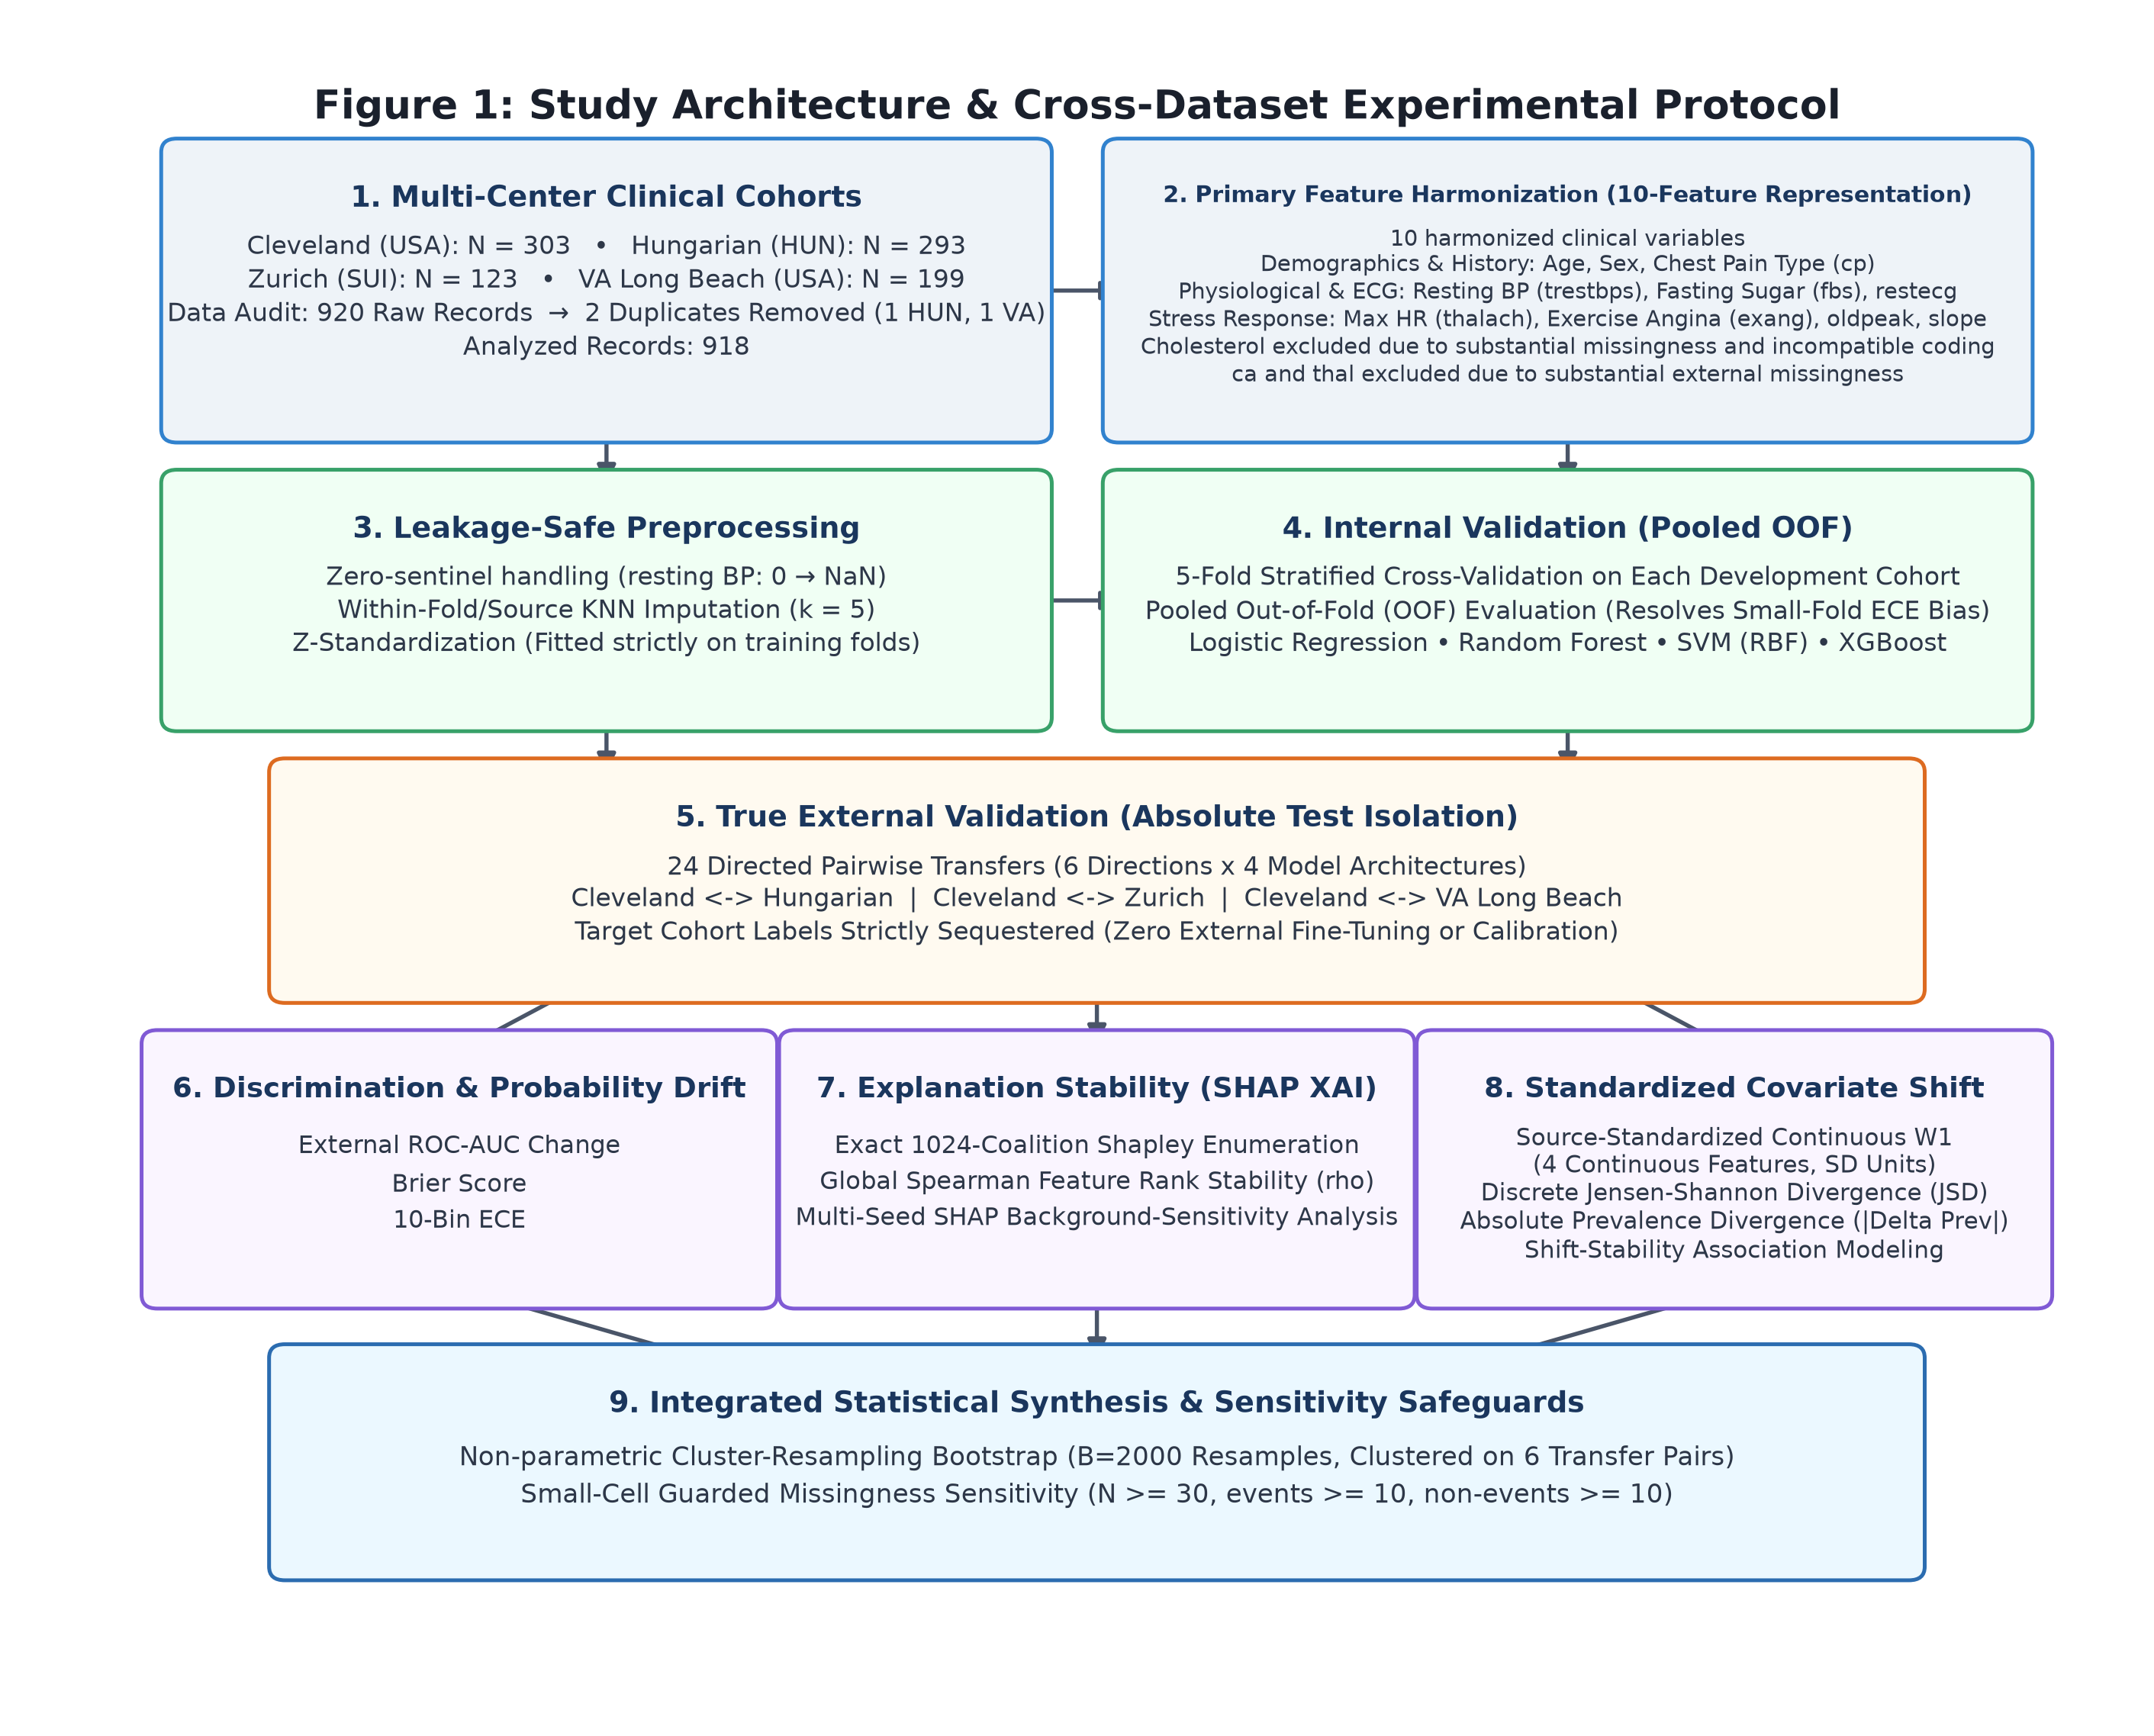
\includegraphics[
        width=0.90\textwidth,
        keepaspectratio
    ]{01_methodological_architecture.png}
    \caption{
        Study architecture and cross-dataset experimental protocol.
        The framework includes cohort harmonization, leakage-safe preprocessing,
        internal validation, true external validation, explanation-stability
        analysis, calibration and dataset-shift analysis, subgroup robustness,
        and integrated statistical synthesis.
    }
    \label{fig:methodology}
\end{figure*}

\subsection{Clinical Cohorts}

Four historical clinical cohorts were obtained directly from the Heart Disease collection of the UCI Machine Learning Repository~\parencite{uciheart}: Cleveland Clinic Foundation, Hungarian Institute of Cardiology, University Hospitals of Zurich and Basel, and Veterans Affairs Medical Center, Long Beach. The corresponding processed UCI files were \texttt{processed.cleveland.data}, \texttt{processed.hungarian.data}, \texttt{processed.switzerland.data}, and \texttt{processed.va.data}. The original clinical study underlying these cohorts was reported by \textcite{detrano1989}. The raw datasets contained 303, 294, 123, and 200 records, respectively; after removal of one exact duplicate in the Hungarian cohort and one in the VA cohort, 918 records remained for analysis.

The primary analysis used a common 10-feature representation:

\begin{equation}
\begin{aligned}
X = \{&
\mathrm{age},\mathrm{sex},\mathrm{cp},\mathrm{trestbps},\mathrm{fbs},\\
&\mathrm{restecg},\mathrm{thalach},\mathrm{exang},
\mathrm{oldpeak},\mathrm{slope}\}.
\end{aligned}
\label{eq:feature_set}
\end{equation}

Cholesterol was excluded because of substantial missingness and incompatible coding patterns across external cohorts. The variables \texttt{ca} and \texttt{thal} were also excluded from the primary representation because of substantial external missingness. The target was harmonized to a binary outcome representing absence or presence of heart disease; Cleveland, Zurich, and VA ordinal targets were converted to zero versus one-or-more disease categories, while the processed Hungarian file was already binary.

\begin{table}[!t]
\centering
\caption{Harmonized clinical cohorts used in the study.}
\label{tab:cohorts}
\small
\setlength{\tabcolsep}{10pt}
\begin{tabular}{lrr}
\toprule
\textbf{Cohort} & \textbf{N} & \textbf{Positive (\%)} \\
\midrule
Cleveland & 303 & 45.9 \\
Hungarian & 293 & 36.2 \\
Zurich/Switzerland & 123 & 93.5 \\
Long Beach VA & 199 & 74.4 \\
\bottomrule
\end{tabular}
\end{table}

\subsection{Leakage-Safe Preprocessing}

Raw datasets were preserved without modification. The zero sentinel for resting blood pressure was treated as missing, whereas valid zero values in other variables were retained. K-nearest-neighbour imputation and standardization were fitted only on development data. For internal validation they were fitted within training folds; for external validation they used training-cohort parameters. Target-cohort observations were therefore transformed without fitting preprocessing parameters to target labels or distributions.

\subsection{Machine Learning Models}

Four classifiers were evaluated: Logistic Regression (LR), Random Forest (RF), Support Vector Machine with an RBF kernel (SVM), and XGBoost. These represent linear, ensemble-tree, kernel-based, and gradient-boosting approaches.

\subsection{Internal Validation}

Five-fold stratified cross-validation was performed independently within each cohort. Out-of-fold predictions were retained for performance and calibration assessment. Metrics included ROC-AUC, precision-recall AUC, Brier score, and expected calibration error (ECE).

\subsection{True External Validation}

The primary external-validation experiment consisted of six directed cohort-transfer directions:

\[
\begin{array}{lll}
\text{Cleveland}\rightarrow\text{Hungarian},&
\text{Cleveland}\rightarrow\text{Zurich},&
\text{Cleveland}\rightarrow\text{VA},\\
\text{Hungarian}\rightarrow\text{Cleveland},&
\text{Zurich}\rightarrow\text{Cleveland},&
\text{VA}\rightarrow\text{Cleveland}.
\end{array}
\]

With four models, this produced 24 model-transfer experiments, corresponding to four model evaluations within each of six directed cohort-transfer pairs. Thus, the 24 model-transfer experiments represent six transfer environments with four model-level observations per environment. External test labels were not used for preprocessing fitting, hyperparameter selection, threshold optimization, oversampling, or model calibration.

For each external-validation experiment, 95\% confidence intervals for ROC-AUC were obtained using a 1,000-resample non-parametric percentile bootstrap on the target test cohort.

\subsection{Explainability Analysis}

SHAP was used as the primary explanation method. SHAP feature rankings were compared between source and target cohorts using Spearman rank correlation. For SVM, exact 1024-coalition Shapley enumeration was used together with a multi-seed background-sensitivity check. The objective was to determine whether feature-attribution structure remained stable under cross-dataset transport.

\subsection{Dataset Shift and Calibration}

Continuous covariate shift was quantified using source-standardized distribution comparisons and the 1-Wasserstein distance across the four continuous features: age, resting blood pressure, maximum heart rate, and ST depression. For each continuous feature, source and target values were standardized using the source cohort's empirical mean and standard deviation. The resulting feature-level 1-Wasserstein distances were averaged using an unweighted arithmetic mean across the four continuous features, yielding a distance expressed in source-domain standard deviation (SD) units. For consistency with Fig.~\ref{fig:methodology}, this metric is denoted source-standardized continuous $W_1$ in SD units. Categorical distribution changes were summarized using distributional divergence measures, and disease prevalence differences were explicitly quantified between source and target cohorts.

Calibration was evaluated using Brier score, Expected Calibration Error (ECE), calibration-in-the-large (intercept), and calibration slope. Logistic recalibration was specified as
\[
\operatorname{logit}\{P(Y=1)\}=\alpha+\beta\,\operatorname{logit}(\hat{p}),
\]
where $\alpha$ represents calibration-in-the-large and $\beta$ represents the calibration slope, with ideal values of $\alpha=0$ and $\beta=1$. Calibration intercepts and slopes were estimated for each external-validation experiment, with 95\% confidence intervals obtained using 1,000-resample stratified non-parametric bootstrap procedures. Empirical calibration curves used five equal-width probability bins, while ECE used ten equal-width bins.

\subsection{Subgroup and Missingness Analysis}

Predefined sex and age groups were evaluated when each subgroup contained at least 30 observations and both outcome classes were present. Missingness sensitivity used a stricter rule requiring $N\geq30$, at least 10 events, and at least 10 non-events. Complete-case and missingness-indicator approaches were compared with the primary imputation strategy.

\subsection{Integrated Statistical Synthesis}

The integrated analysis used the 24 model-transfer experiments clustered within six directed cohort-transfer pairs. A non-parametric cluster-resampling block bootstrap with $B=2000$ resamples with replacement, clustered on the six directed transfer pairs, was used for uncertainty estimation. Confidence intervals were calculated using empirical 2.5th and 97.5th percentiles of the bootstrap distribution. Associations were interpreted descriptively rather than causally.

% ============================================================
% IV. RESULTS
% ============================================================

\section{Results}

\subsection{Cohort Characteristics}

The cohorts differed substantially in sample size and disease prevalence (Table~\ref{tab:cohorts}). These differences provide an important basis for evaluating transportability because external performance was assessed without rebalancing or tuning the target cohort. Pooled out-of-fold internal validation results for all four models and cohorts are summarized in Table~\ref{tab:internal_validation}.

Internal validation performance varied substantially across cohorts. Cleveland and Hungarian showed relatively high discrimination across the four models, whereas performance was lower in the Zurich and VA Long Beach cohorts. In particular, the Zurich SVM yielded an ROC-AUC of 0.465, while the other Zurich models ranged from 0.590 to 0.658. These estimates should be interpreted cautiously because the Zurich cohort contained only eight negative observations and therefore provides limited information for discrimination assessment.

Because disease prevalence in the Zurich cohort was 93.5\%, the corresponding PR-AUC values should not be interpreted independently of this high-prevalence setting.

\begin{table}[!b]
\centering
\caption{Pooled out-of-fold internal validation results.}
\label{tab:internal_validation}
\scriptsize
\setlength{\tabcolsep}{6pt}
\begin{tabular}{llrrrr}
\toprule
\textbf{Cohort} & \textbf{Model} & \textbf{AUC (\%)} & \textbf{PR-AUC (\%)} & \textbf{Brier} & \textbf{ECE} \\
\midrule
Cleveland & LR  & 86.87 & 86.35 & 0.1449 & 0.0518 \\
           & RF  & 86.52 & 85.94 & 0.1487 & 0.0390 \\
           & SVM & 86.59 & 86.38 & 0.1441 & 0.0461 \\
           & XGB & 85.74 & 84.02 & 0.1544 & 0.0500 \\
\midrule
Hungarian & LR  & 89.21 & 84.85 & 0.1176 & 0.0308 \\
          & RF  & 88.45 & 82.91 & 0.1263 & 0.0320 \\
          & SVM & 87.86 & 83.54 & 0.1280 & 0.0479 \\
          & XGB & 88.86 & 84.45 & 0.1245 & 0.0454 \\
\midrule
Zurich & LR  & 59.02 & 95.16 & 0.0820 & 0.0592 \\
       & RF  & 62.07 & 96.58 & 0.0665 & 0.0757 \\
       & SVM & 46.52 & 93.91 & 0.0683 & 0.0283 \\
       & XGB & 65.76 & 96.68 & 0.0657 & 0.0566 \\
\midrule
VA Long Beach & LR  & 69.97 & 85.24 & 0.1732 & 0.0772 \\
              & RF  & 66.37 & 82.35 & 0.1789 & 0.0467 \\
              & SVM & 63.60 & 81.86 & 0.1808 & 0.0829 \\
              & XGB & 65.48 & 81.41 & 0.1862 & 0.0925 \\
\bottomrule
\end{tabular}
\end{table}

\subsection{External Discrimination Performance}

Figure~\ref{fig:external_auc} summarizes ROC-AUC across the 24 external-validation experiments.

\begin{figure}[!t]
    \centering
    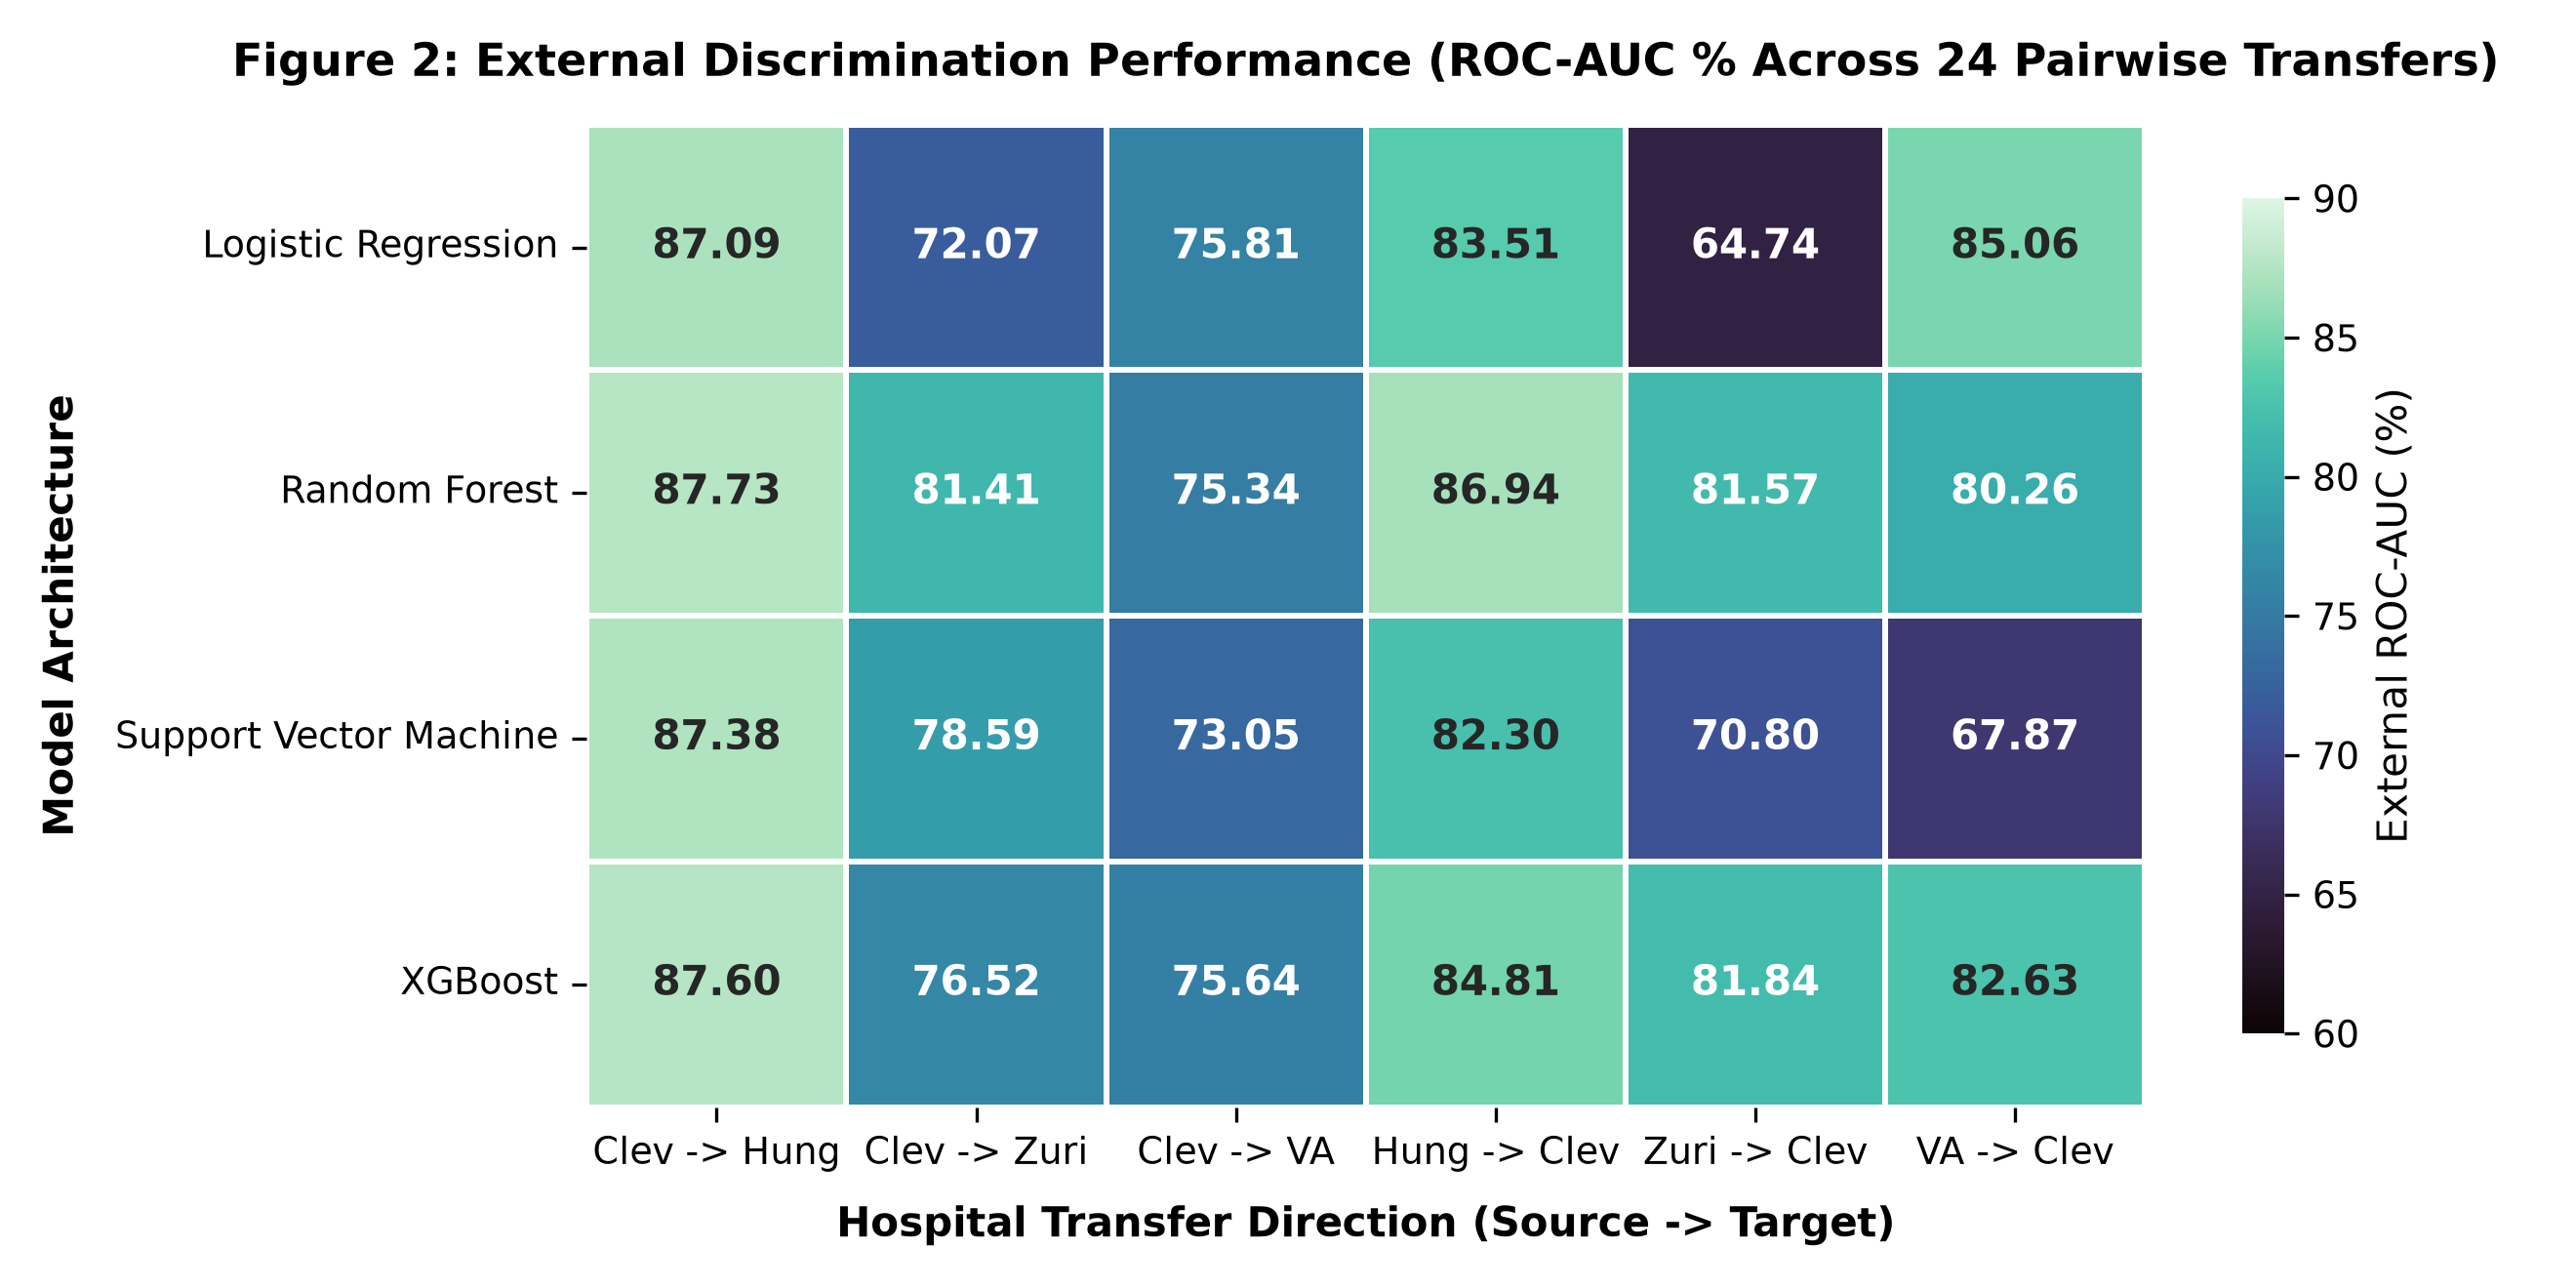
\includegraphics[
        width=\columnwidth,
        keepaspectratio
    ]{02_external_validation_auc_heatmap.png}
    \caption{
        External discrimination performance across 24 pairwise transfer
        experiments. Each cell represents ROC-AUC for a specific model
        and directed source-to-target cohort transfer.
    }
    \label{fig:external_auc}
\end{figure}

Cleveland-to-Hungarian transfers produced ROC-AUC values of 87.09\% (95\% CI: 82.55--91.23\%), 87.73\% (95\% CI: 83.28--91.68\%), 87.38\% (95\% CI: 83.39--91.29\%), and 87.60\% (95\% CI: 83.14--91.65\%) for Logistic Regression, Random Forest, SVM, and XGBoost, respectively. Cleveland-to-Zurich produced ROC-AUC values of 72.07\%, 81.41\%, 78.59\%, and 76.52\%, while Cleveland-to-VA produced 75.81\%, 75.34\%, 73.05\%, and 75.64\%.

In the reverse direction, Hungarian-to-Cleveland produced 83.51\%, 86.94\%, 82.30\%, and 84.81\%. Zurich-to-Cleveland ranged from 64.74\% to 81.84\%, while VA-to-Cleveland ranged from 67.87\% to 85.06\%. The confidence intervals were particularly wide for transfers into the Zurich cohort, consistent with the small number of negative observations in that cohort. Thus, discrimination varied according to transfer direction and cohort rather than following a uniform degradation pattern.

\FloatBarrier

\subsection{Calibration and Dataset Shift}

Calibration error and discrimination did not change in parallel. Figure~\ref{fig:calibration} illustrates calibration and external ECE.

\begin{figure}[!t]
    \centering
    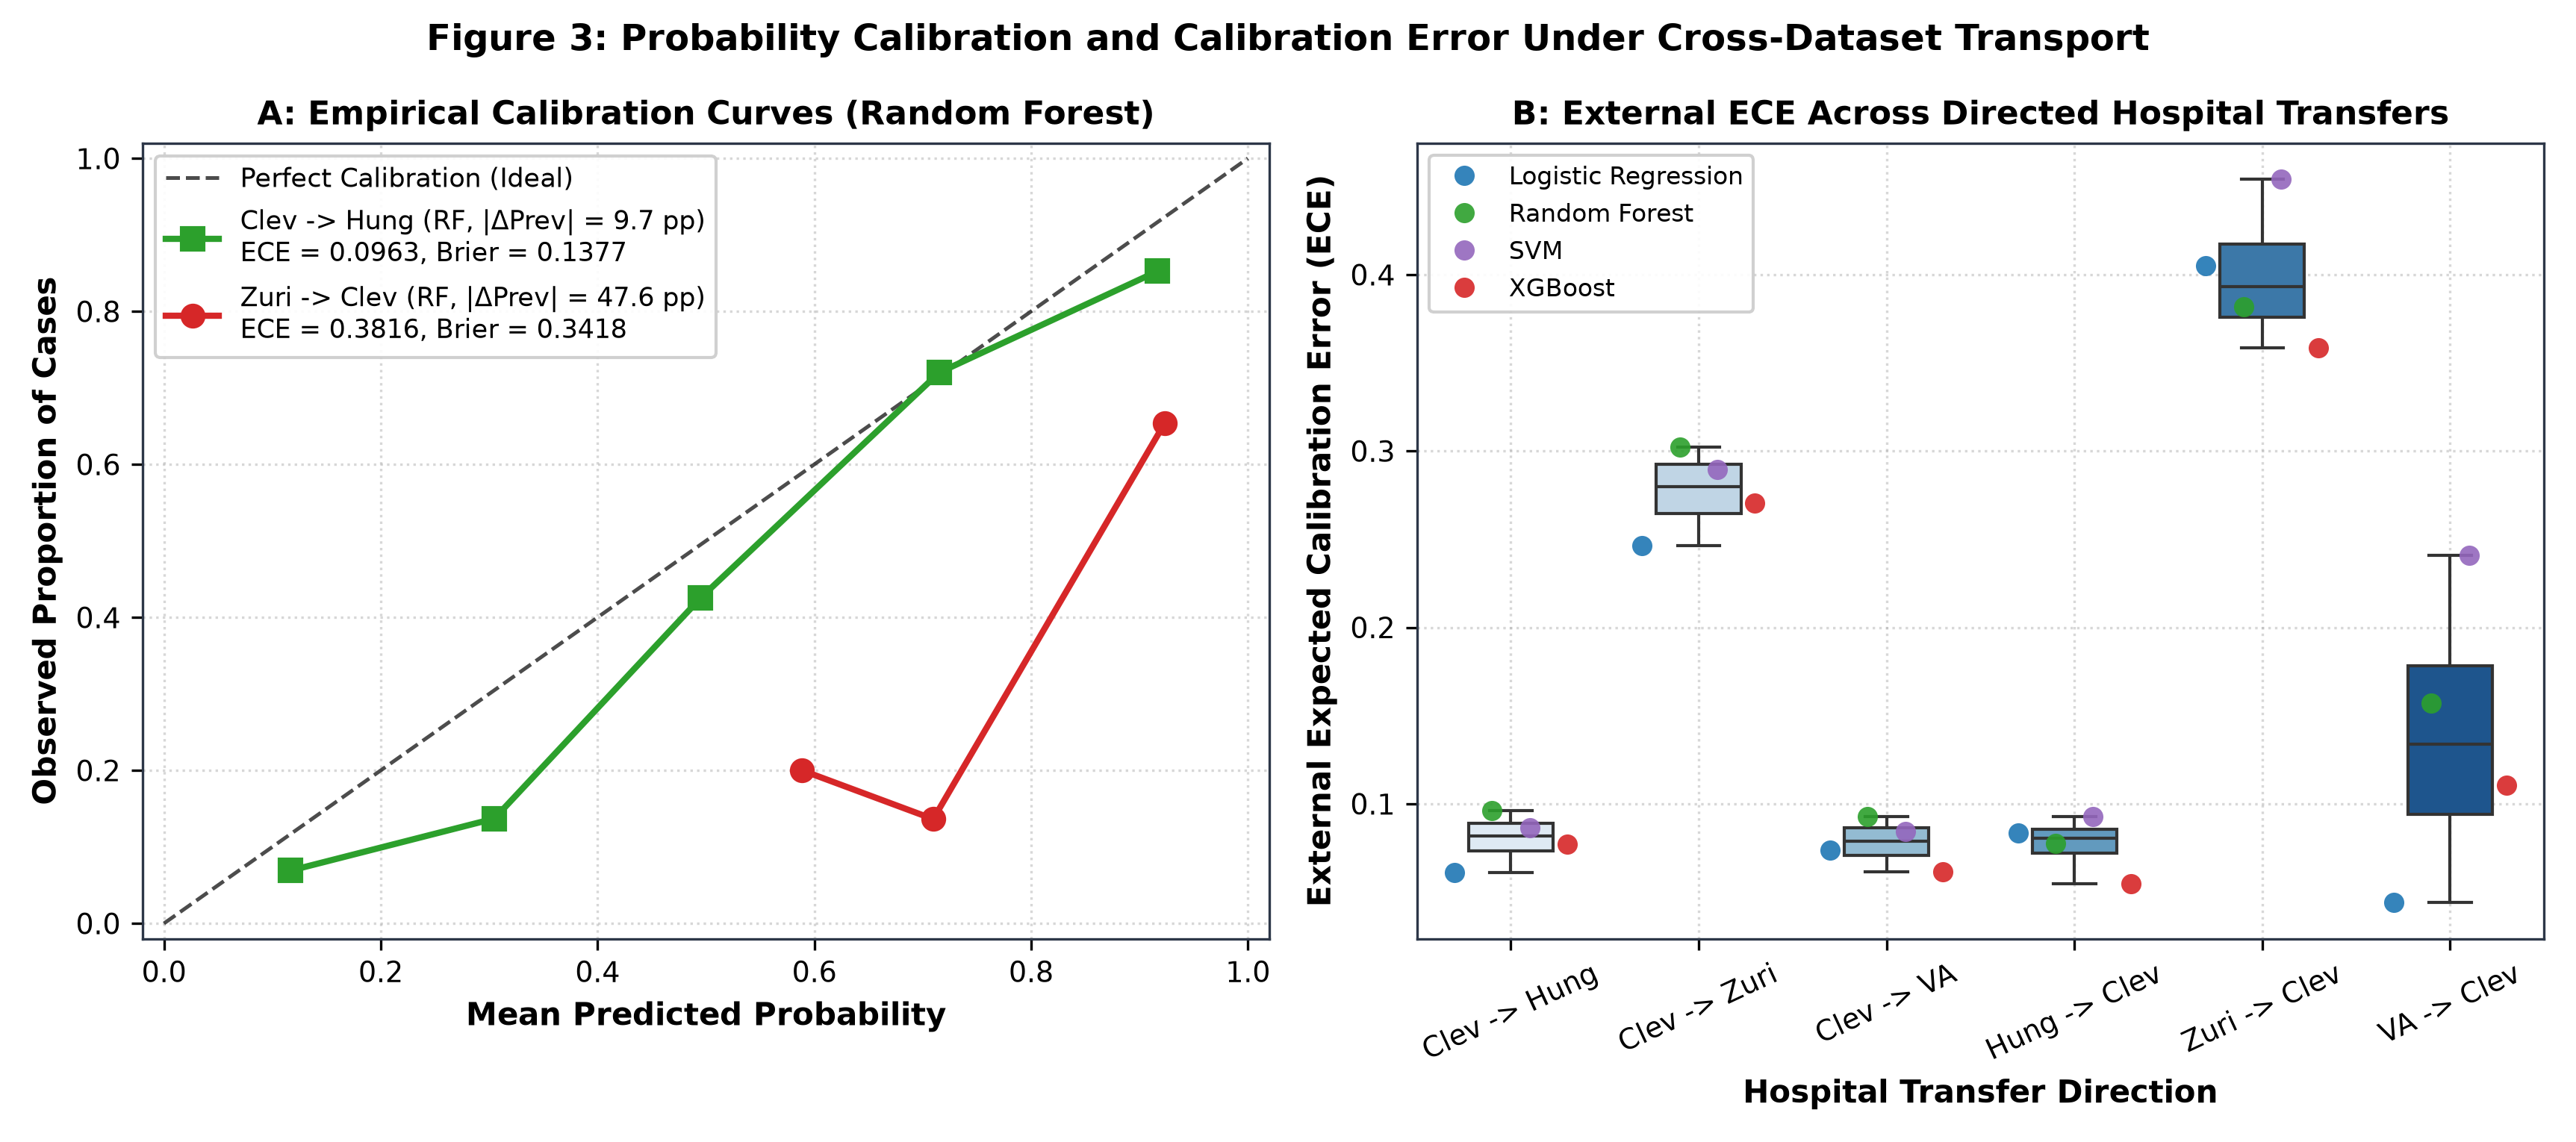
\includegraphics[
        width=\columnwidth,
        keepaspectratio
    ]{03_calibration_dataset_shift.png}
    \caption{
        Probability calibration and calibration error under cross-dataset
        transport. Panel A compares empirical calibration for Random Forest
        in Cleveland-to-Hungarian and Zurich-to-Cleveland transfers. Panel B
        summarizes external ECE across the six directed transfer directions.
    }
    \label{fig:calibration}
\end{figure}

For Cleveland-to-Hungarian Random Forest, ECE was 0.0963 and Brier score was 0.1377. The calibration-in-the-large intercept was $-0.54$ (95\% CI: $-0.73$ to $-0.37$), while the calibration slope was $1.09$ (95\% CI: $0.86$ to $1.39$). In contrast, Zurich-to-Cleveland Random Forest showed ECE of 0.3816 and Brier score of 0.3418, with a calibration-in-the-large intercept of $-2.26$ (95\% CI: $-2.38$ to $-2.13$) and a calibration slope of $0.91$ (95\% CI: $0.59$ to $1.36$). The prevalence difference between Cleveland and Hungarian was approximately 9.7 percentage points, compared with 47.6 percentage points between Zurich and Cleveland.

\FloatBarrier

\subsection{Explanation Stability}

SHAP rank stability across the 24 primary transfers is shown in Fig.~\ref{fig:shap_stability}.

\begin{figure}[!t]
    \centering
    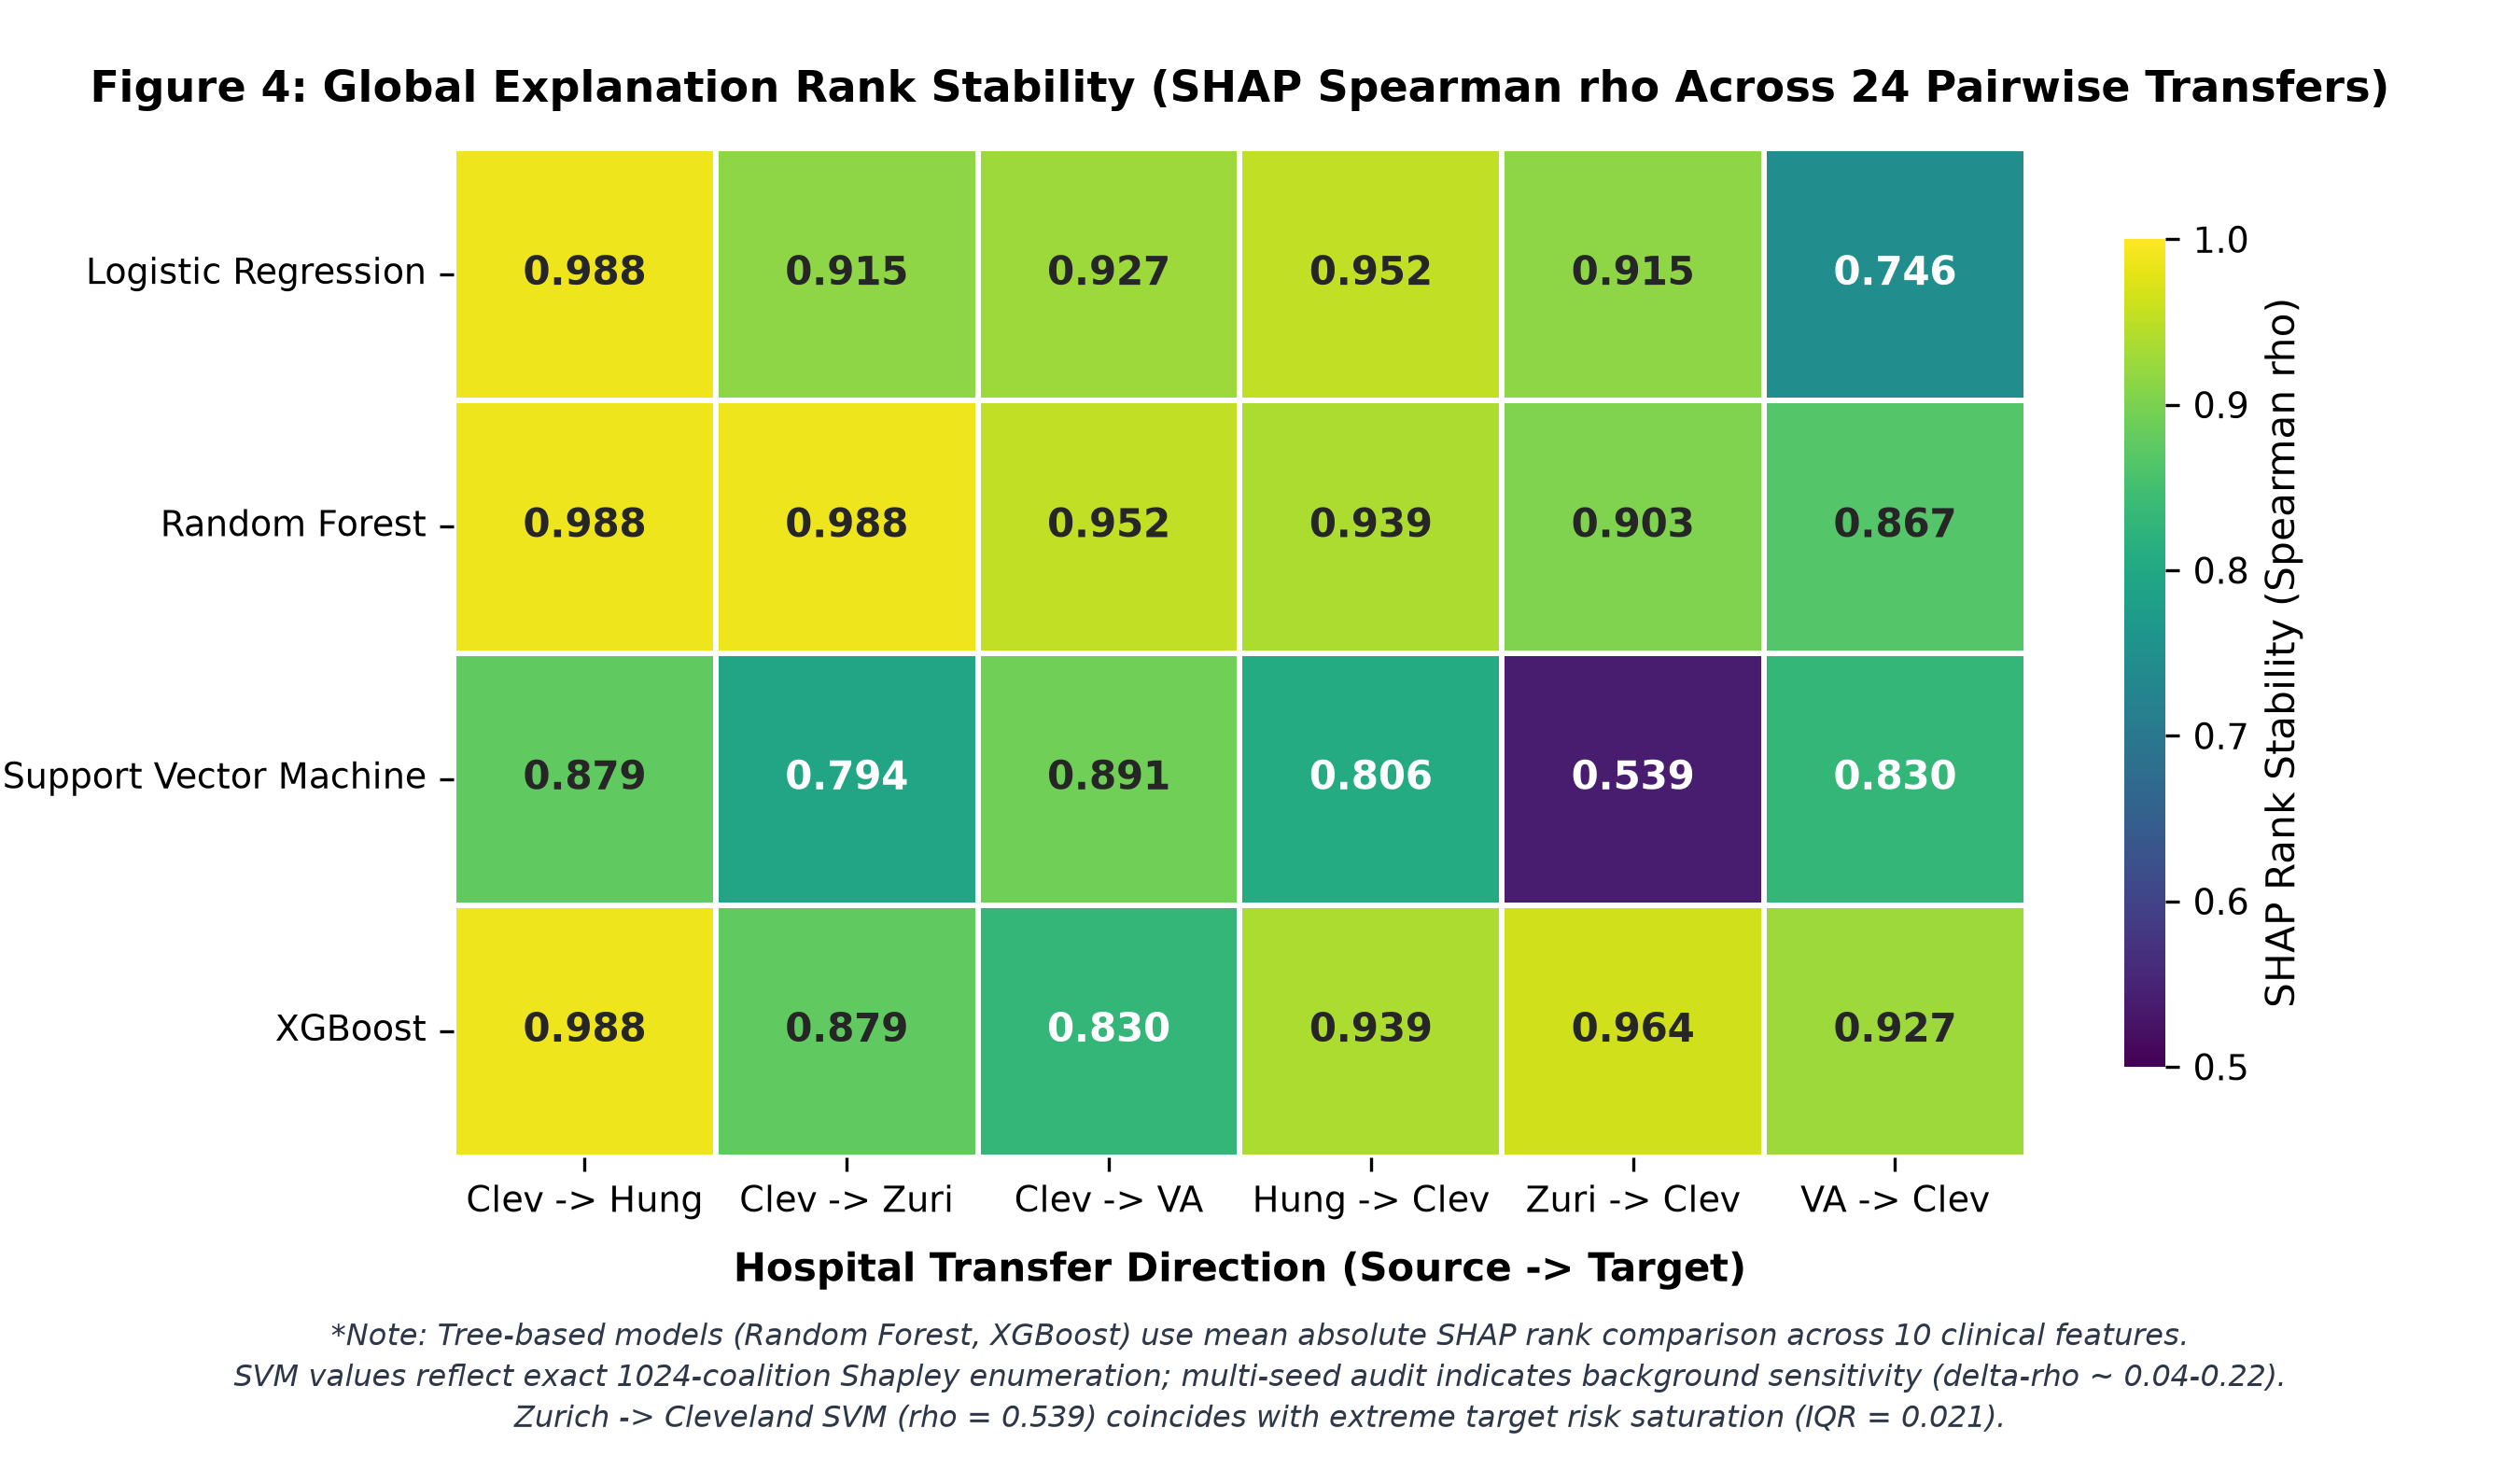
\includegraphics[
        width=\columnwidth,
        keepaspectratio
    ]{04_shap_explanation_stability.png}
    \caption{
        Global explanation-rank stability across 24 directed cross-dataset
        transfer experiments. Values represent Spearman rank correlation
        between source- and target-cohort SHAP feature-importance rankings.
    }
    \label{fig:shap_stability}
\end{figure}

Several transfers showed high SHAP rank correlations. For Cleveland-to-Hungarian, correlations were 0.988, 0.988, 0.879, and 0.988 for LR, RF, SVM, and XGBoost, respectively. Lower stability was observed in selected transfers, including Zurich-to-Cleveland SVM, with a correlation of 0.5394. SVM background-sensitivity analysis showed changes across seeds in the approximate range of 0.04--0.22.

\FloatBarrier

\subsection{Dataset Shift and Explanation Stability}

Figure~\ref{fig:shift_shap} presents the relationship between standardized Wasserstein feature shift and SHAP explanation stability.

\begin{figure}[!t]
    \centering
    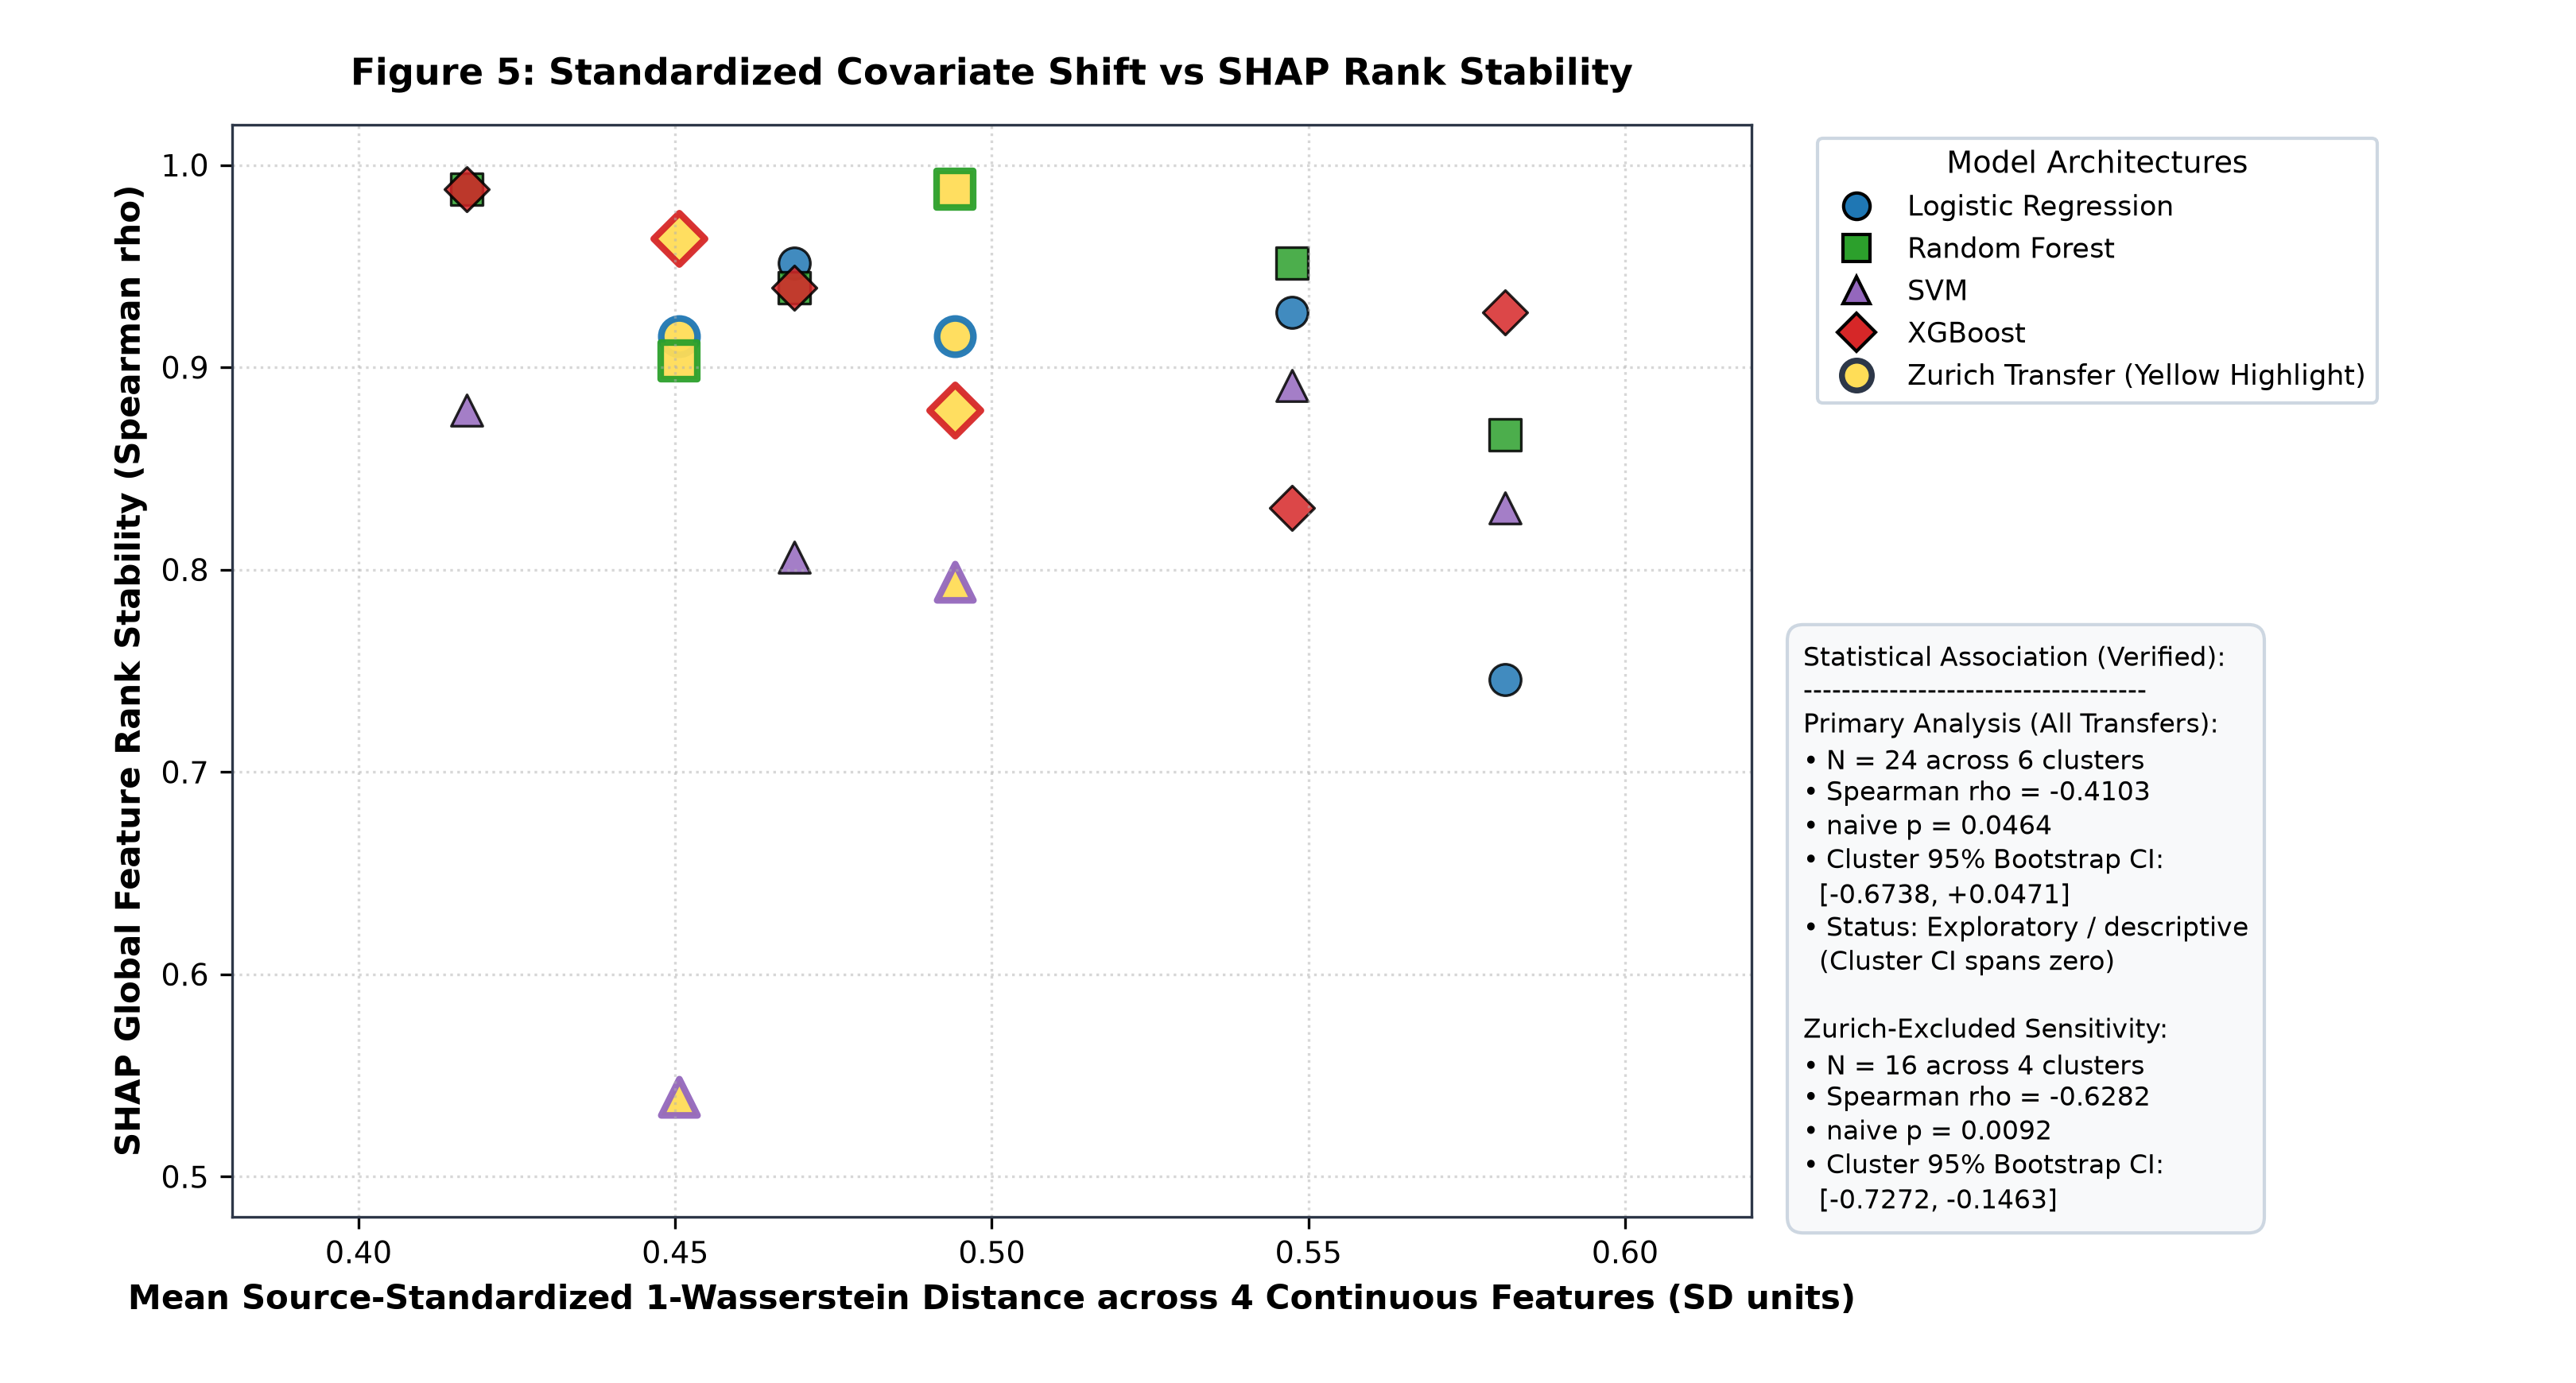
\includegraphics[
        width=\columnwidth,
        keepaspectratio
    ]{05_dataset_shift_vs_shap_stability.png}
    \caption{
        Association between standardized continuous covariate shift and
        SHAP explanation rank stability. The relationship is descriptive;
        all 24 model-transfer experiments are shown and clustered by
        directed transfer pair.
    }
    \label{fig:shift_shap}
\end{figure}

Across all 24 experiments, the Spearman association between mean standardized Wasserstein shift and SHAP rank stability was $\rho=-0.4103$ (naive $p=0.0465$), with a cluster-aware 95\% bootstrap confidence interval of $[-0.6738,+0.0471]$. When Zurich-related transfers were excluded, the association was $\rho=-0.6282$ ($p=0.0092$), with a cluster-aware 95\% confidence interval of $[-0.7272,-0.1463]$. Because the primary cluster-aware interval spans zero, these associations are interpreted as exploratory and descriptive.

\FloatBarrier

\subsection{Subgroup Robustness and Missingness}

Figure~\ref{fig:subgroup} summarizes the evaluated subgroup disparities and missingness sensitivity.

\begin{figure}[!t]
    \centering
    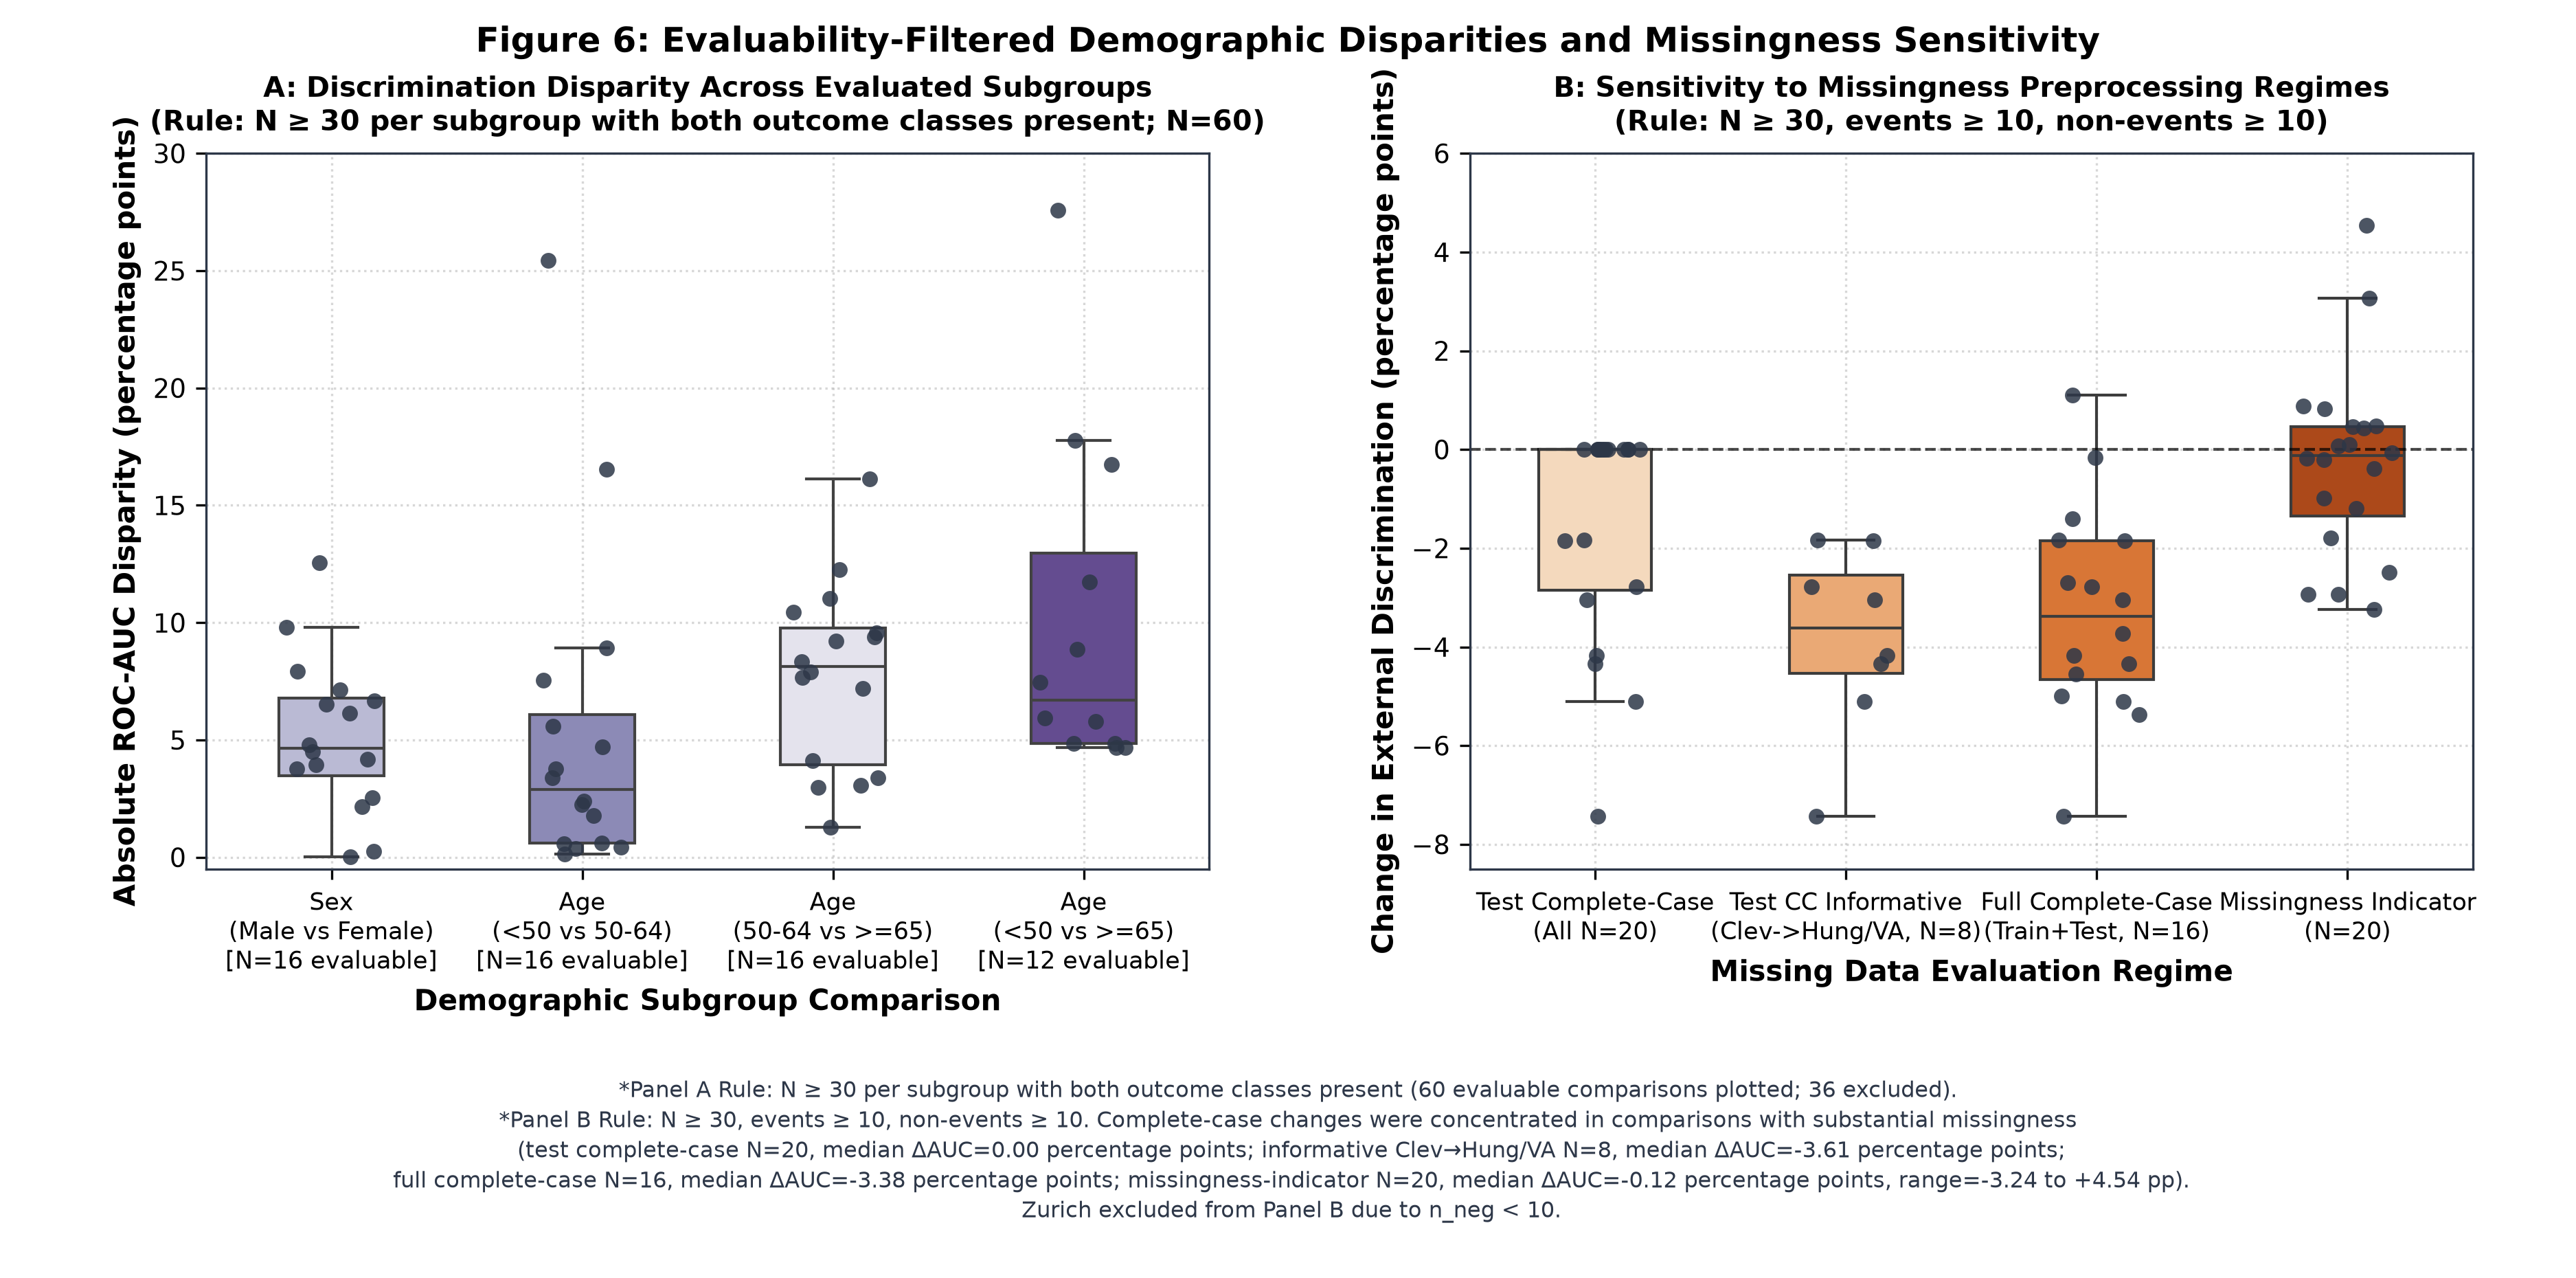
\includegraphics[
        width=\columnwidth,
        keepaspectratio
    ]{06_subgroup_or_missingness_robustness.png}
    \caption{
        Evaluability-filtered demographic subgroup disparities and missingness
        sensitivity. Panel A uses $N\geq30$ per subgroup with both outcome
        classes present. Panel B uses $N\geq30$, events $\geq10$, and
        non-events $\geq10$.
    }
    \label{fig:subgroup}
\end{figure}

The final demographic-subgroup evaluability filter retained 60 comparisons and excluded 36. Missingness sensitivity showed a zero-heavy distribution under test complete-case analysis. Here, $\Delta$AUC denotes the difference in ROC-AUC between the missingness-sensitive analysis and the corresponding primary analysis. Across 20 comparisons, the median $\Delta$AUC was 0.00 percentage points, with 12 structural zeros. Among eight informative Cleveland-to-Hungarian and Cleveland-to-VA complete-case comparisons, the median $\Delta$AUC was $-3.61$ percentage points, ranging from $-7.43$ to $-1.83$ percentage points. Full train-and-test complete-case analysis ($N=16$) produced a median $\Delta$AUC of $-3.38$ percentage points. The missingness-indicator approach ($N=20$) produced a median of $-0.12$ percentage points, ranging from $-3.24$ to $+4.54$ percentage points.

The demographic subgroup analysis showed that subgroup disparities were heterogeneous across the evaluated comparisons rather than exhibiting a consistent direction across cohorts and models. These results provide additional context for the aggregate external-validation estimates and indicate that model performance may vary across patient subgroups within a cohort.

\FloatBarrier

% ============================================================
% V. INTEGRATED STATISTICAL SYNTHESIS
% ============================================================

\section{Integrated Statistical Synthesis}

The full analysis showed a descriptive association between absolute prevalence divergence and external ECE, with Spearman $\rho=0.7593$ and a cluster-aware 95\% bootstrap confidence interval of $[0.1206,0.8706]$. Excluding Zurich-related experiments reduced this association to $\rho=0.1898$. The Wasserstein-shift association with SHAP stability was $\rho=-0.4103$ in the primary analysis, with a cluster-aware confidence interval spanning zero; the Zurich-excluded sensitivity analysis produced $\rho=-0.6282$. The association between SHAP stability and $\Delta$AUC was weak ($\rho=-0.0868$).

Because the 24 experiments are clustered within six directed transfer pairs, these relationships are treated as exploratory and descriptive rather than as confirmatory estimates based on 24 independent populations. Overall, discrimination, calibration, and explanation stability represent related but non-equivalent dimensions of model reliability.

% ============================================================
% VI. DISCUSSION
% ============================================================

\section{Discussion}

This study examined whether explainable heart disease models remain reliable when transported to different clinical cohorts. External-validation results demonstrated substantial heterogeneity between transfer directions rather than a uniform change in discrimination. This indicates that transportability depends on the relationship between the model and target population.

Calibration provided information beyond ROC-AUC. The Zurich cohort had markedly different disease prevalence from Cleveland, and models trained on Zurich produced large calibration errors when evaluated on Cleveland. These results support evaluating probability calibration alongside discrimination when models are transported between populations.

The explanation analysis adds another dimension. SHAP rankings were highly stable for several transfers but showed lower stability in selected shifted settings. The observed association between standardized Wasserstein shift and SHAP stability was exploratory and did not establish a causal mechanism. Overall, the findings support a multidimensional evaluation framework combining external validation, calibration, dataset shift, explanation stability, subgroup robustness, and missingness sensitivity.

% ============================================================
% VII. LIMITATIONS
% ============================================================

\section{Limitations}

Several limitations should be considered. The analysis relied on historical publicly available datasets that may not represent contemporary clinical populations. The Zurich cohort contained only eight negative observations, limiting precision for some estimates. Cross-dataset experiments were clustered by transfer direction and should not be interpreted as 24 independent patient populations. The cohorts also differ in clinical setting, data collection, coding practices, and variable availability. SHAP explanations should not be interpreted as causal clinical effects. Finally, prospective clinical validation, temporal validation in contemporary populations, decision-curve analysis, and evaluation within real clinical workflows were outside the study scope.

% ============================================================
% VIII. CONCLUSION
% ============================================================

\section{Conclusion}

This study evaluated heart disease prediction models under cross-dataset transport rather than relying exclusively on internal random-split performance. External discrimination, probability calibration, and explanation stability changed differently across transfer directions. Larger prevalence differences coincided with higher external calibration error in the full analysis, although this association was substantially attenuated when Zurich-related experiments were excluded. The primary association between standardized feature-distribution shift and SHAP rank stability was negative but had a cluster-aware confidence interval spanning zero. These findings indicate that reliable clinical machine learning evaluation requires true external validation together with calibration, dataset-shift characterization, explanation-stability analysis, and subgroup and missingness sensitivity.

% ============================================================
% DATA AND CODE AVAILABILITY
% ============================================================

\section*{Data and Code Availability}

The datasets analyzed in this study are publicly available through the UCI Machine Learning Repository Heart Disease dataset \parencite{uciheart}. The repository contains the Cleveland, Hungarian, Switzerland, and VA Long Beach databases. The preprocessing, external-validation, explainability, dataset-shift, calibration, subgroup, and statistical-synthesis code will be made available in a public repository to facilitate reproducibility.

% ============================================================
% ACKNOWLEDGMENT
% ============================================================

\section*{Acknowledgment}

The author acknowledges the open clinical datasets and publicly available research resources that supported this methodological investigation.

% ============================================================
% REFERENCES
% ============================================================

\begingroup
\setlength{\bibitemsep}{0pt}
\setlength{\bibparsep}{0pt}
\printbibliography
\endgroup

\end{document}